\section{Utilisation, production, sources de pollution et types d'environnements contamin\'es}
\subsection{Utilisation}
\par{
La plupart des plastiques, ayant une densit\'e assez faible sont l\'egers. Ils ont des propri\'et\'es thermiques, m\'ecaniques, \'electriques, optiques permettant d'en faire des produits \`a usages divers. Certains peuvent \^etre transparents, permettant de fabriquer des dispositifs optiques. Ils r\'esistent \`a l'action corrosive de nombreuses substances. On peut les mouler facilement dans des formes complexes, permettant d'int\'egrer diff\'erentes mati\`eres et fonctions. De plus, en vue d'am\'eliorer ou modifier certaines de leurs propri\'et\'es physiques, on peut y ajouter des mati\`eres de renforcement, des colorants, des retardateurs de flamme, des plastifiants, afin de r\'epondre aux besoins d'une application donn\'ee. Le secteur des emballages est le plus gros consommateur de plastique. Plus de 50\% des marchandises en Europe sont emball\'ees dans du plastique {\citep{Plasticseurope2}}.
}
\par{
Une part importante de l'utilisation du plastique concerne le secteur de l'emballage , mais aussi celui du b\^atiment, des transports, de l'\'electricit\'e et d'autres usages vari\'es comme le mat\'eriel de sports et de loisirs {\citep{SCF}}.
}

\begin{figure}[h]
\centering
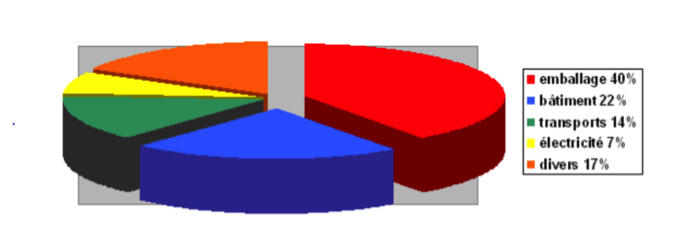
\includegraphics[scale=1]{Secteurs.png}
\caption{Consommation des mati\`eres plastiques selon les secteurs d'utilisation {\citep{SCF}}} 
\label{secteurs}
\end{figure}
\FloatBarrier

\par{
La consommation est diff\'erente selon la forme d'utilisation. Le tableau ci-dessous reprend les diff\'erents types de plastique et leurs formes d'utilisation les plus courantes:
}

\begin{table}[h]
\centering
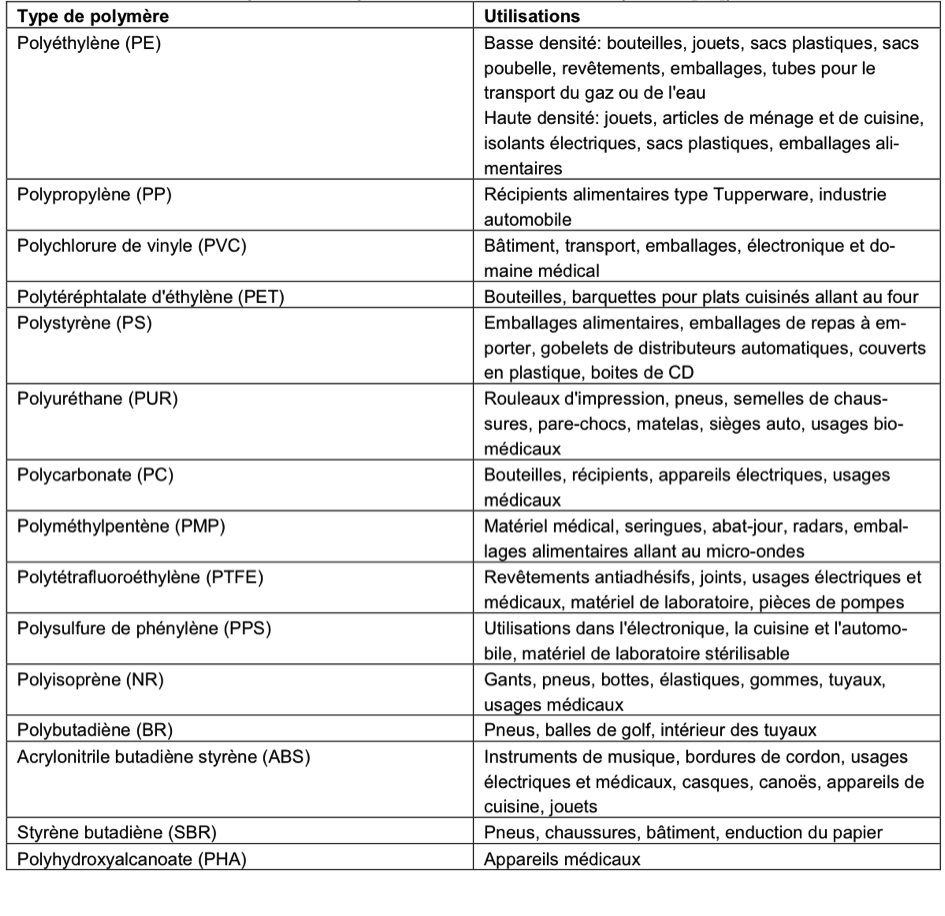
\includegraphics[scale=1]{Diffpoly.png}
\caption{Les diff\'erents types de polym\`eres et leurs principales utilisations {\citep{Schafer2015}}} 
\label{diffpoly}
\end{table}
\FloatBarrier

\subsection{Production du plastique}
\par{
La  quantit\'e  de  plastique  produite  dans  le  monde  est  pass\'ee de 230 \`a 322 millions de tonnes par an en dix ans {\citep{Plasticseurope}} consommant 8\% environ de la production mondiale de p\'etrole {\citep{Planetoscope}}. Le vapocraquage est un proc\'ed\'e p\'etrochimique qui consiste \`a obtenir, \`a partir d'une coupe p\'etroli\`ere telle que le naphta, des alc\`enes qui sont \`a la base de l'industrie des mati\`eres plastiques produisant ainsi le poly\'ethyl\`ene ou le polypropyl\`ene par exemple {\citep{Europetrole}}.
}

\begin{figure}[h]
\centering
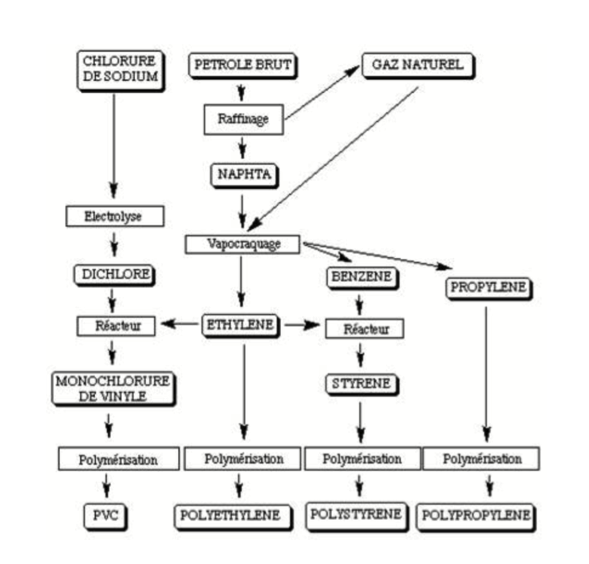
\includegraphics[scale=1]{Fabrication.png}
\caption{Modes de fabrication des principaux thermoplastiques {\citep{SCF}}} 
\label{fabrication}
\end{figure}
\FloatBarrier
